\documentclass{anstrans} \usepackage{amsmath} \usepackage{amssymb}
%\usepackage{amsthm}
\usepackage{amscd}
%\usepackage{amsfonts}
\usepackage{graphicx}% \usepackage{fancyhdr} \usepackage{color} \usepackage{cite}

%\usepackage[T1]{fontenc} \usepackage[utf8]{inputenc} \usepackage{authblk}
\usepackage{physics} \usepackage{float} \usepackage{caption} \usepackage{subcaption}

\setlength{\columnsep}{0.5 in}

\newcommand{\expv}[1]{\ensuremath{\mathbb{E}[ #1]}} \newcommand{\xs}[2]{\ensuremath{\Sigma_{#1}^{(#2)}}}
\newcommand{\intO}{\ensuremath{\int\limits_{4\pi}}} \newcommand{\intz}{\ensuremath{\int\limits_0^1}}
\newcommand{\intf}{\ensuremath{\int\limits_{-\infty}^\infty}}
\newcommand{\intzf}{\ensuremath{\int\limits_{0}^\infty}}
\newcommand{\LargerCdot}{\raisebox{-0.25ex}{\scalebox{1.2}{$\cdot$}}}

%\textwidth6.6in \textheight9in


%\setlength{\topmargin}{0.3in} \addtolength{\topmargin}{-\headheight} \addtolength{\topmargin}{-\headsep}

%\setlength{\oddsidemargin}{0in}

%\oddsidemargin  0.0in \evensidemargin 0.0in \parindent0em

%\pagestyle{fancy}\lhead{MATH 579 (UQ for PDEs)} \rhead{02/24/2014} \chead{Project Proposal} \lfoot{}
%\rfoot{\bf \thepage} \cfoot{}
\title{Adaptive Sparse-Grid Stochastic Collocation Uncertainty Quantification Convergence for Multigroup
Diffusion}

\author{Paul W. Talbot$^{*}$, Anil K. Prinja$^{*}$, Cristian Rabiti$^{\dagger}$} \institute{$^*$Department of
Nuclear Engineering, University of New Mexico, Albuquerque, NM, 87131 \and $^\dagger$Nuclear Engineering
Methods Development, Idaho National Laboratory, Idaho Falls, ID, 834115} \email{talbotp@unm.edu \and
prinja@unm.edu \and cristian.rabiti@inl.gov}
%\date{}


\begin{document} \section{Introduction} Advanced methods in  uncertainty quantification for numerical models
in computational physics \cite{SCLagrange}\cite{textbook} continue to gain acceptance in nuclear
modeling \cite{Ayres}\cite{ayres2}.  Previously, we demonstrated the efficiency of sparse-grid stochasatic
collocation in comparison with Monte Carlo for uncertainty quantification through convergence studies
\cite{ans2014}.  We consider an adaptive method for anisotropic sparse grid collocation and its convergence
compared to previous efforts.

The physical system we consider is a two-dimensional quarter-core reactor, consisting of 5 materials
distributed in 121 regions (see Fig. \ref{geom}).  We solve the two-group neutron diffusion criticality
approximation \begin{align} -\grad\cdot\qty( D_1(\bar x)\grad\phi_1(\bar x))+&\qty(\xs{a}{1}(\bar
  x)+\xs{s}{1\to2}(\bar x))\phi_1(\bar x) \nonumber\\ &= \frac{1}{k(\phi)}\sum_{g'=1}^2\nu_{g'}\xs{f}{g'}(\bar
  x)\phi_{g'}(\bar x), \end{align} \begin{equation} -\grad \cdot\qty(D_2(\bar x)\grad \phi_2(\bar
  x))+\xs{a}{2}(\bar x)\phi_2(\bar x) = \xs{s}{1\to 2}(\bar x)\phi_1(\bar x).  \end{equation} We apply vacuum
boundaries on the top and right, and reflecting boundaries on the bottom and left.  The criticality eigenvalue
and quantity of interest $k(\phi)$ is given by \begin{equation}
  k(\phi)=\sum_{g=1}^2\iint\limits_D\frac{\nu\xs{f}{g}\phi_g(\bar x)}{\qty(-\nabla\cdot
    D_g\nabla+\Sigma_r^{(g)})\phi_g(\bar x)}~d\bar x.  \end{equation} The material properties are shown in
  Table \ref{tab:coremats}, and the domain is $[0,200\text{ cm}]^2$.  The reference value
  $k$=1.00007605445.  \begin{figure}[H] \centering 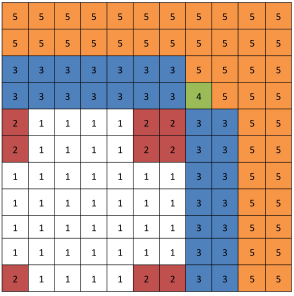
\includegraphics[width=0.5\linewidth]{../graphics/core}
    \caption{Core Geometry} \label{geom} \end{figure} \begin{table}[h] \centering \begin{tabular}{c c | c c c
      c} Mat. & $g$ & $D_g$ & $\Sigma_{a,g}$ & $\nu\Sigma_{f,g}$ & $\Sigma_s^{1,2}$ \\ \hline 1 & 1 & 1.255 &
      8.252e-3 & 4.602e-3 & 2.533e-2 \\ & 2 & 2.11e-1 & 1.003e-1 & 1.091e-1 & \\ \hline 2 & 1 & 1.268 &
      7.181e-3 & 4.609e-3 & 2.767e-2 \\ & 2 & 1.902e-1 & 7.047e-2 & 8.675e-2 & \\ \hline 3 & 1 & 1.259 &
      8.002e-3 & 4.663e-3 & 2.617e-2 \\ & 2 & 2.091e-1 & 8.344e-2 & 1.021e-1 & \\ \hline 4 & 1 & 1.259 &
      8.002e-3 & 4.663e-3 & 2.617e-2 \\ & 2 & 2.091e-1 & 7.3324e-2 & 1.021e-1 & \\ \hline 5 & 1 & 1.257 &
      6.034e-4 & 0 & 4.754e-2 \\ & 2 & 1.592e-1 & 1.911e-2 & 0 & \end{tabular} \caption{Reference Material
    Properties for Benchmark Core} \label{tab:coremats} \end{table}

The material cross sections, neutron multiplication factors, and diffusion coefficients are potential
uncertain input parameters.  We introduce uniformly-distributed uncertainty within 5\% of the reference
values.  The uncertain distributions make up the uncertainty space $\Gamma\subset\mathbb{R}^N,$ where $N$ is
the number of uncertain parameters.
We consider the input parameter uncertainties to be independently distributed.

\section{Methods}
%\subsection{Deterministic Space}
We solve our system of equations by imposing a mesh grid on the physical domain using the local and global
particle-conserving finite volume method.  We solve the system of equations nonlinearly with the criticality
eigenvalue, using Jacobian-free Newton-Krylov methods.  We use the GMRES algorithm in the \texttt{trilinos}
solver package.% from Sandia National Laboratory \cite{Trilinos-Overview}.  

Developing an adaptive algorithm for uncertainty quantification builds on the sparse grid formulation used 
previously \cite{ans2014} and
analysis of variance \cite{Ayres}.  We represent the $k$-eigenvalue as a function of input parameters as
$u(Y)$.  The generalized polynomial chaos expansion is given by
\begin{equation}\label{approx}
  u(Y)\approx u_{h}(Y)=\sum_{k=0}^\eta c_k\Phi_k(Y),
\end{equation} 
\begin{equation} 
  \Phi_k(Y)=\prod_{n=1}^N \phi_{k_n}(Y_n), 
\end{equation} 
%\begin{equation} 
%  \mathcal{L}_{k_n}(Y_n)=\prod_{j=1}^i\frac{Y_n-Y_n^{(i)}}{Y_n^{(k_n)}-Y_n^{(i)}}, 
%\end{equation} 
where $u_h(Y)$ is the
spatially-discretized PDE solution, and $\phi_{k_n}(y_n)$ are Askey polynomials of order $k_n$ that are
orthonormal with respect to the probability distribution function $\rho_n(y_n)$ over the probability space
$\Omega$.
Using orthonormality, we obtain an expression for the expansion coefficients $c_k$ as
\begin{equation}
  c_k = \langle u(Y)\Phi(Y)\rangle = \int_\Omega u(Y)\Phi(Y)\rho(Y) dY.
\end{equation}
Because $Y$ are uniformly distributed, we use Gauss-Legendre quadrature to obtain
collocation points and weights to evaluate $c_k$.  %The order of the quadrature is obtained based on polynomial expansion orders
%from a polynomial index set $\Lambda(L)$.  
%For a single uncertain parameter ($N=1$) and a fourth-order polynomial
%approximation ($L=4$), $\Lambda$ includes all polynomial orders from 0 to 4 $\qty(\Lambda=[0,1,2,3,4])$.  Each
%index point $p\in\Lambda$ corresponds to a polynomial expansion moment of order $p$.

Previously we identified static methods to determine the index set $\Lambda$ \cite{ans2014}.  We propose an
adaptive method based on analysis of variance to construct the index set, following a pattern similar to the
algorithm in \cite{Ayres}.  A property of the gPC expansion is the method of calculating variance, namely
\begin{equation}
  \sigma^2 = \expv{u_h(Y)^2} - \expv{u_h(Y)}^2 = \sum_{k\in\Lambda}c_k^2 - c_0^2.
\end{equation}
The partial percent variance $\eta$ due to each polynomial is
\begin{equation}
  \eta_k \equiv \frac{c_k^2}{\sigma^2}.
\end{equation}
The adaptive method is initialized by evaluating the gPC to a first-order polynomial expansion in each
dimension.  The algorithm then continues by searching the polynomial indices that may be added to the index
set, which is dependent on the existing polynomials.  The admissibility condition is
\begin{equation}
  k-e_j\in\Lambda \text{  for } 1\leq j\leq N, k_j>1,
\end{equation}
where $e_j$ is a unit vector in the direction $j$.  The estimated partial variance for a prospective polynomial 
is the product of immediate subset polynomials,
\begin{equation}
  \tilde \eta_k = \prod_{j=1,k_j>0}^N \eta_{k_j-e_j}.
\end{equation}
The adaptive algorithm chooses the prospective polynomial with the largest estimated partial variance to add
to the index set, and the algorithm continues until estimated remaining variance is less than tolerance.
%%%%OLD%%%%%%

\section{Results}\label{results}
%\subsection{Stochastic Convergence} We vary the number of uncertain inputs including
\begin{table}[H] \centering \begin{tabular}{c|c|c} Material & Property & Distribution \\ \hline Material 1 &
    $\nu\Sigma_{2,f}$ & $\mathcal{U}(0.0981,0.1201)$ \\ Material 1 & $\Sigma_{2,c}$ &
    $\mathcal{U}(0.0499,0.0609)$  \\ Material 4 & $\nu\Sigma_{2,f}$ & $\mathcal{U}(0.0921,0.1121)$ \\ Material
    4 & $\Sigma_{2,c}$ & $\mathcal{U}(0.03732,0.04552)$  \\ Material 5 & $D_2$ & $\mathcal{U}(0.1432,0.1752)$
  \end{tabular} \caption{Uncertain Input Parameters} \label{params} \end{table}

We obtain the error in the moments $r$ of the quantity of interest $k(Y)=u(Y)$, given by
\begin{equation}
  \epsilon_h^{(r)}=\frac{|\expv{u_h^{(r)}}-\expv{u_\text{ref}^{(r)}}|}{\expv{u_\text{ref}^{(r)}}},
\end{equation}
\begin{equation}
  \expv{u_h^{(r)}}=\expv{S_{N,\Lambda_\text{TD}(L)}[u_h](Y)^{(r)}}=\sum_{k=1}^\eta w_k
  ~u_h^{(r)}\qty(Y^{(k)}).
\end{equation}

%%%%%%%%%%%%%%%%%%%%%%%
TODO WORKING HERE
%%%%%%%%%%%%%%%%%%%%%%%
Figs. \ref{n1mean}-\ref{n5var} show the comparison of Monte Carlo convergence to stochastic collocation for
$N=1,3,5$ where $N$ is the number of uncertain parameters.  Both total degree (TD) and hyperbolic cross (HC)
index sets have been included for $N>1$ (they are indistinguishable for $N=1$).

Because of the regularity of $k(Y)=u(Y)$, the total degree index set is as cost-effective as the hyperbolic
cross index set.  For a less regular stochastic solution, we expect hyperbolic cross would be more efficient.
We also expect the convergence rate to diminish with increasing $N$, and that trend can be seen in the figures
for the mean and variance of $k(Y)$. Both the magnitude of the error as well as the convergence rate of
stochastic collocation outperforms Monte Carlo for any number of runs.  In addition, heuristic selection of
importance weighting improved the accuracy of sparse grid methods by approximately half an order of magnitude.
%\begin{figure}[H] \centering \begin{subfigure}[b]{0.24 \textwidth}
%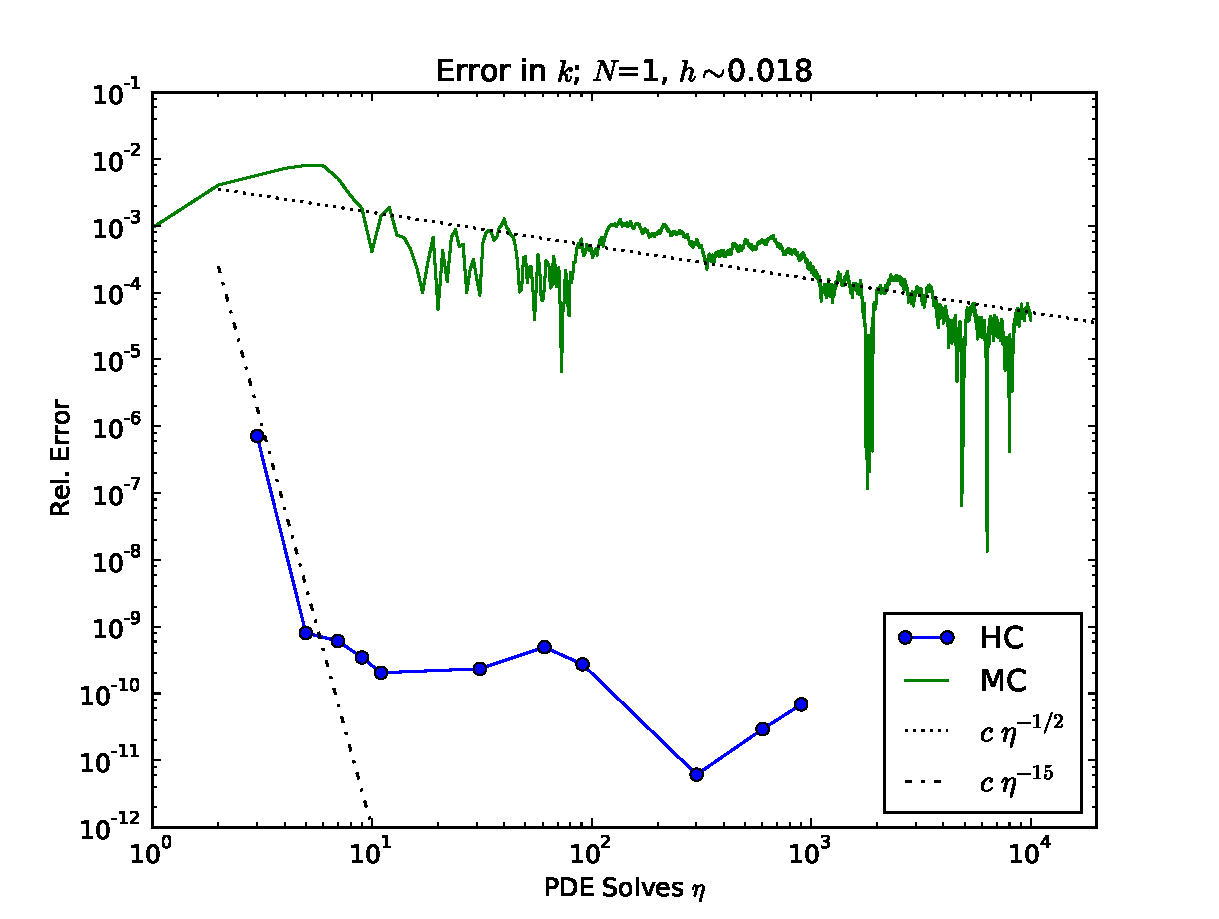
\includegraphics[width=\textwidth]{N1_h5_MCHC} \caption{Mean} \label{n1mean} \end{subfigure}
%\begin{subfigure}[b]{0.24 \textwidth} 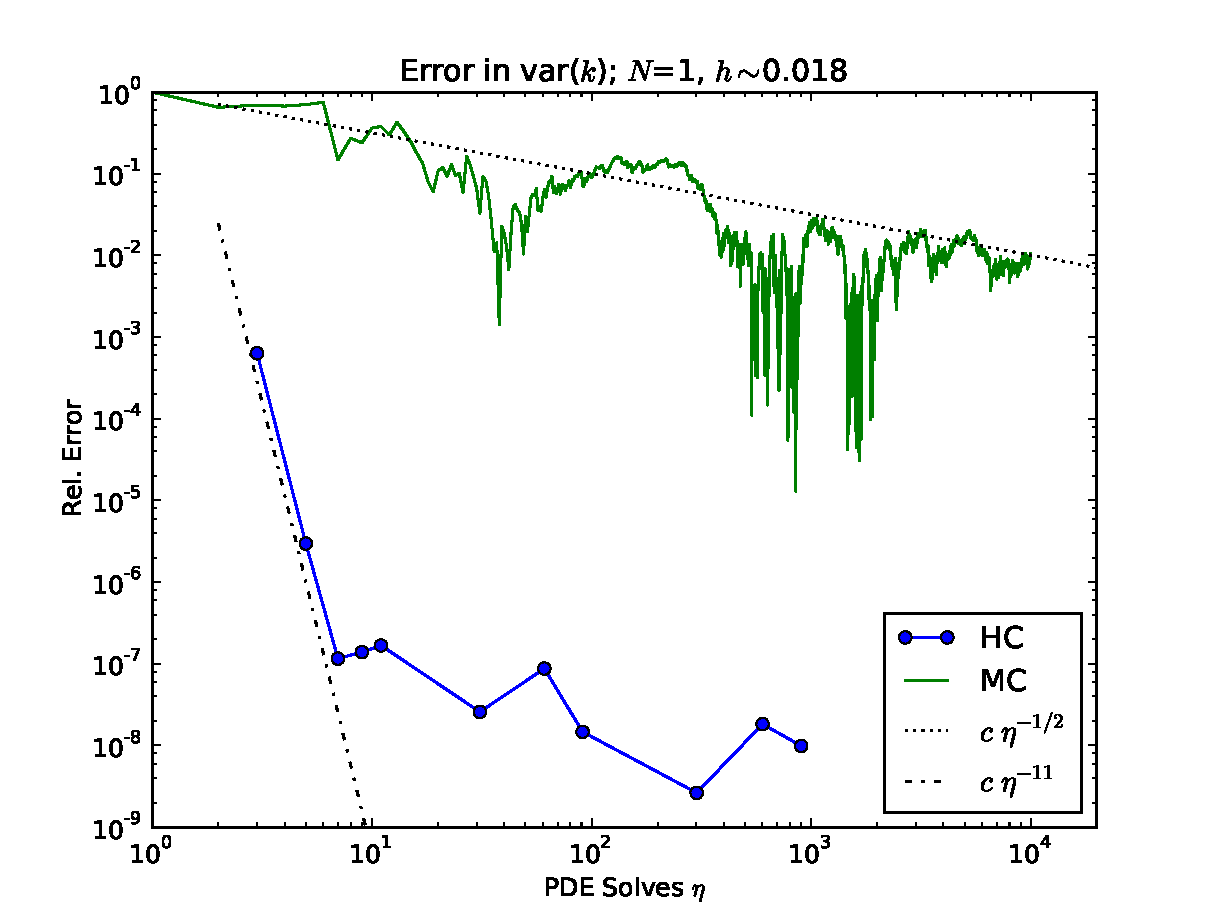
\includegraphics[width=\textwidth]{N1_h5_MCHC_2} \caption{Variance}
%\label{n1var} \end{subfigure} \caption{$N=1$} \label{n1} \end{figure}
%
%\begin{figure}[H] \centering \begin{subfigure}[b]{0.24 \textwidth}
%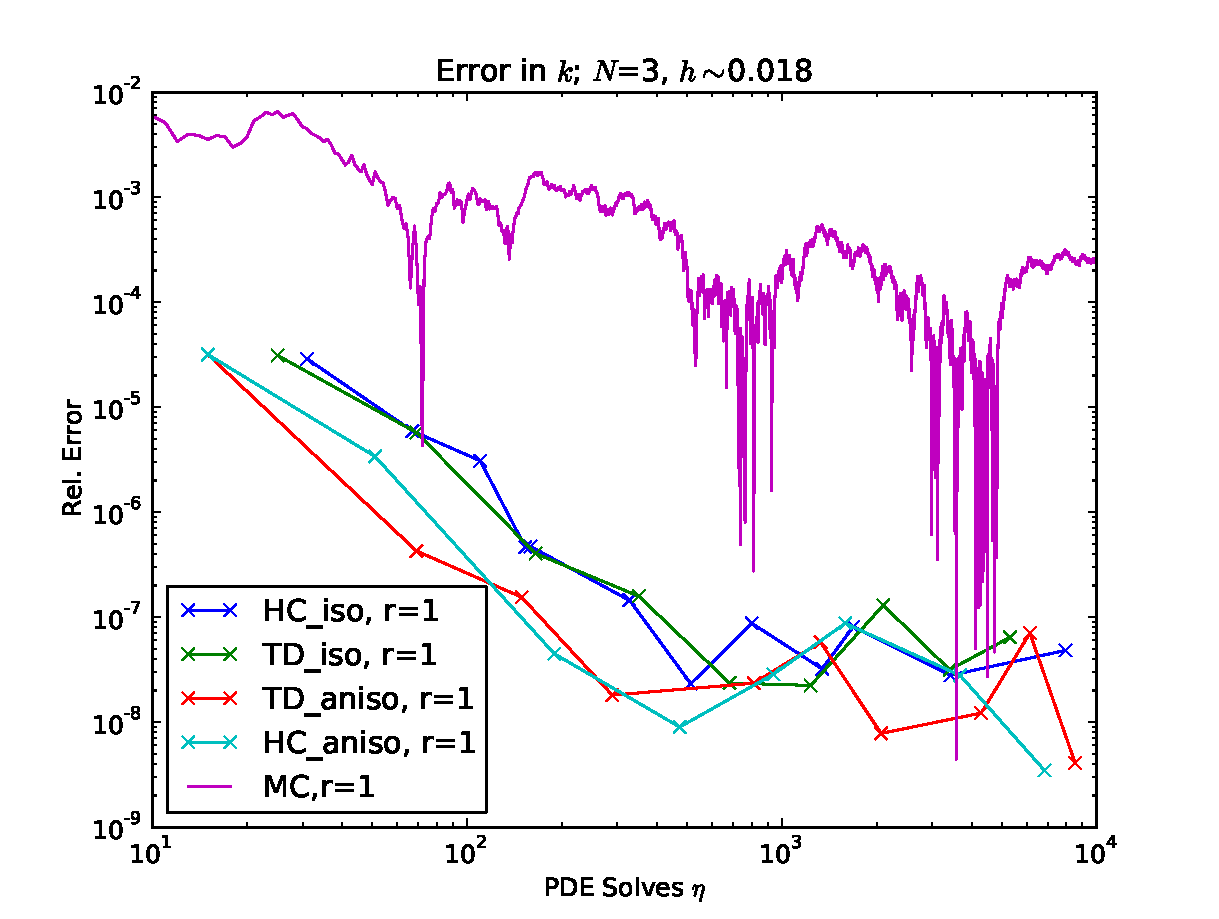
\includegraphics[width=\textwidth]{N3_h5_MCHC} \caption{Mean} \label{n3mean} \end{subfigure}
%\begin{subfigure}[b]{0.24 \textwidth} 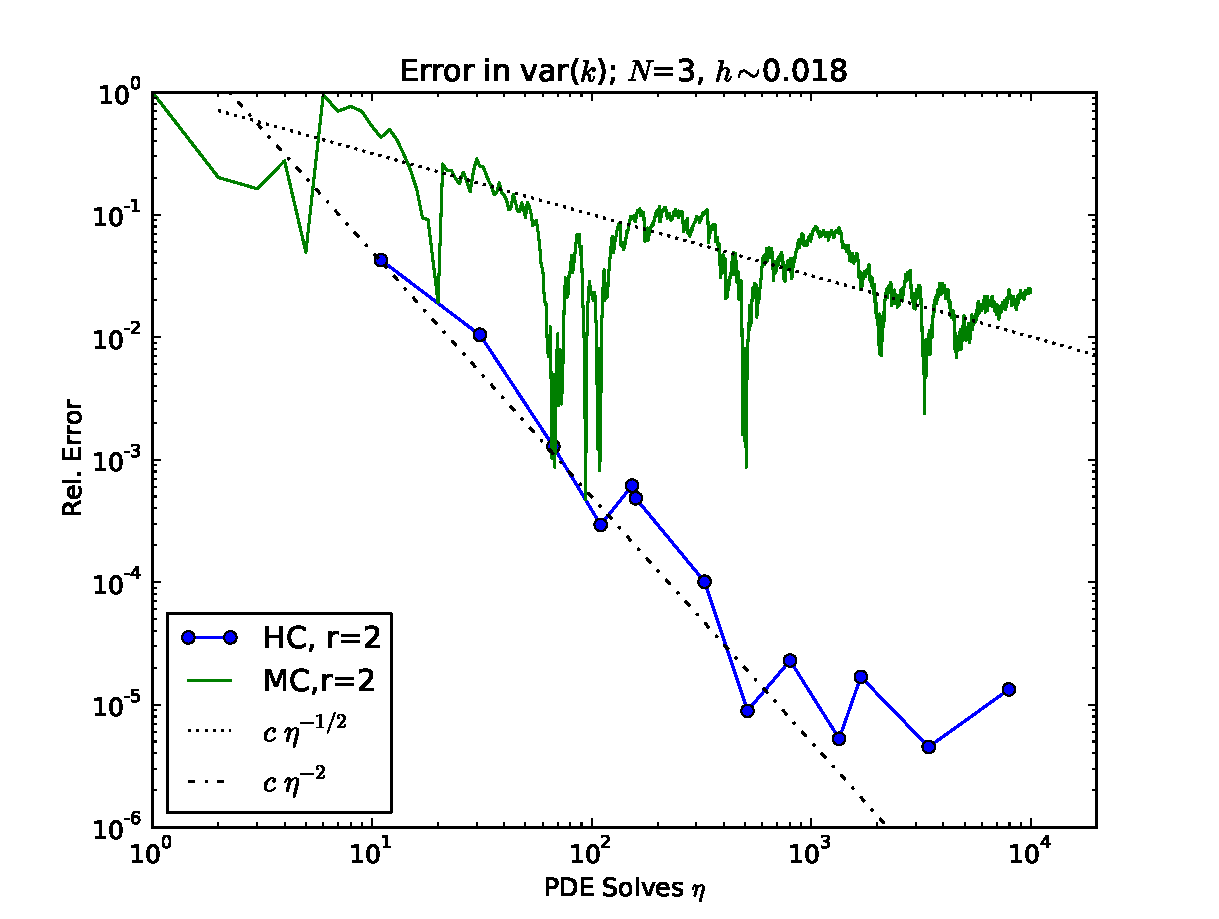
\includegraphics[width=\textwidth]{N3_h5_MCHC_2} \caption{Variance}
%\label{n3var} \end{subfigure} \caption{$N=3$} \label{n3} \end{figure}
%
%\begin{figure}[H] \centering \begin{subfigure}[b]{0.24 \textwidth}
%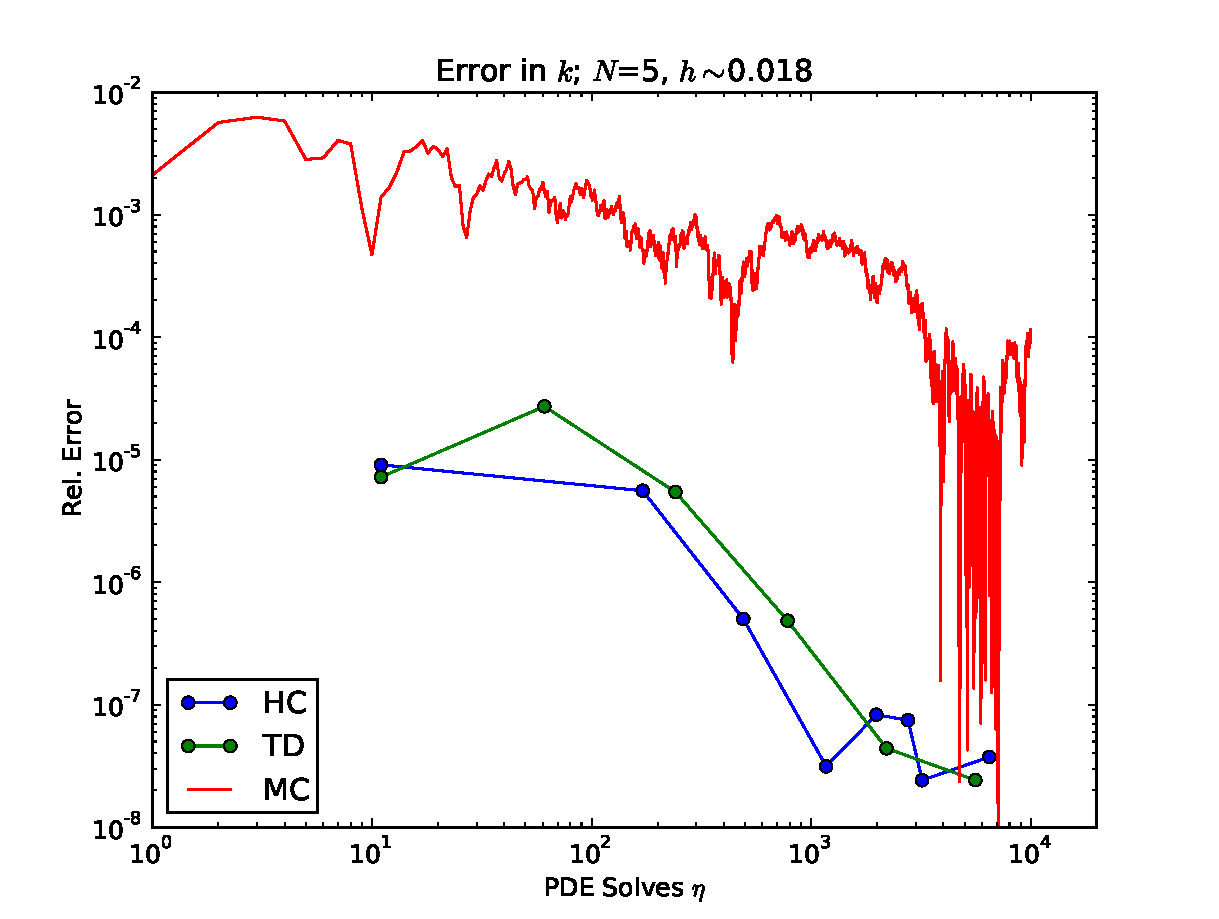
\includegraphics[width=\textwidth]{N5_h5_MCHC} \caption{Mean} \label{n5mean} \end{subfigure}
%\begin{subfigure}[b]{0.24 \textwidth} 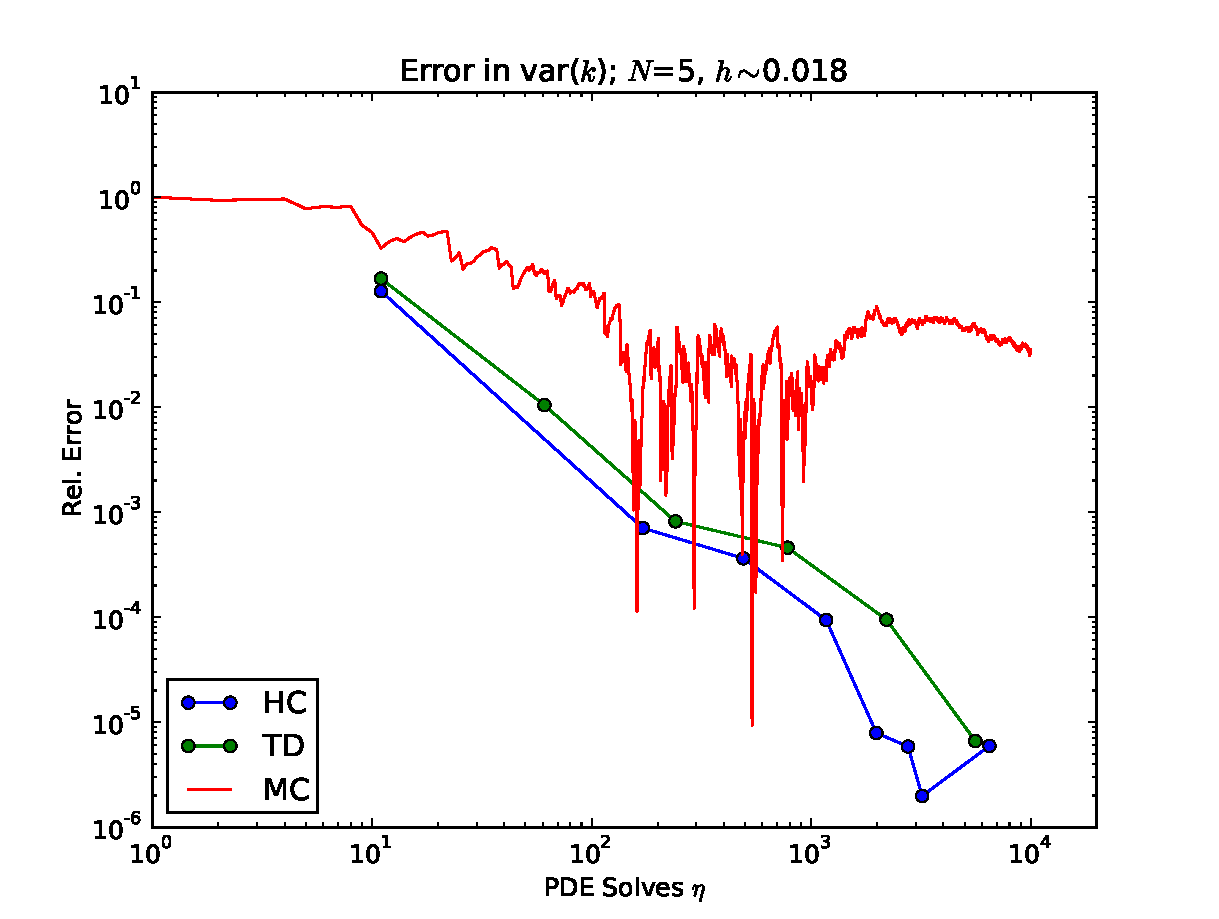
\includegraphics[width=\textwidth]{N5_h5_MCHC_2} \caption{Variance}
%\label{n5var} \end{subfigure} \caption{$N=5$} \label{n5} \end{figure} \begin{figure}[H]
%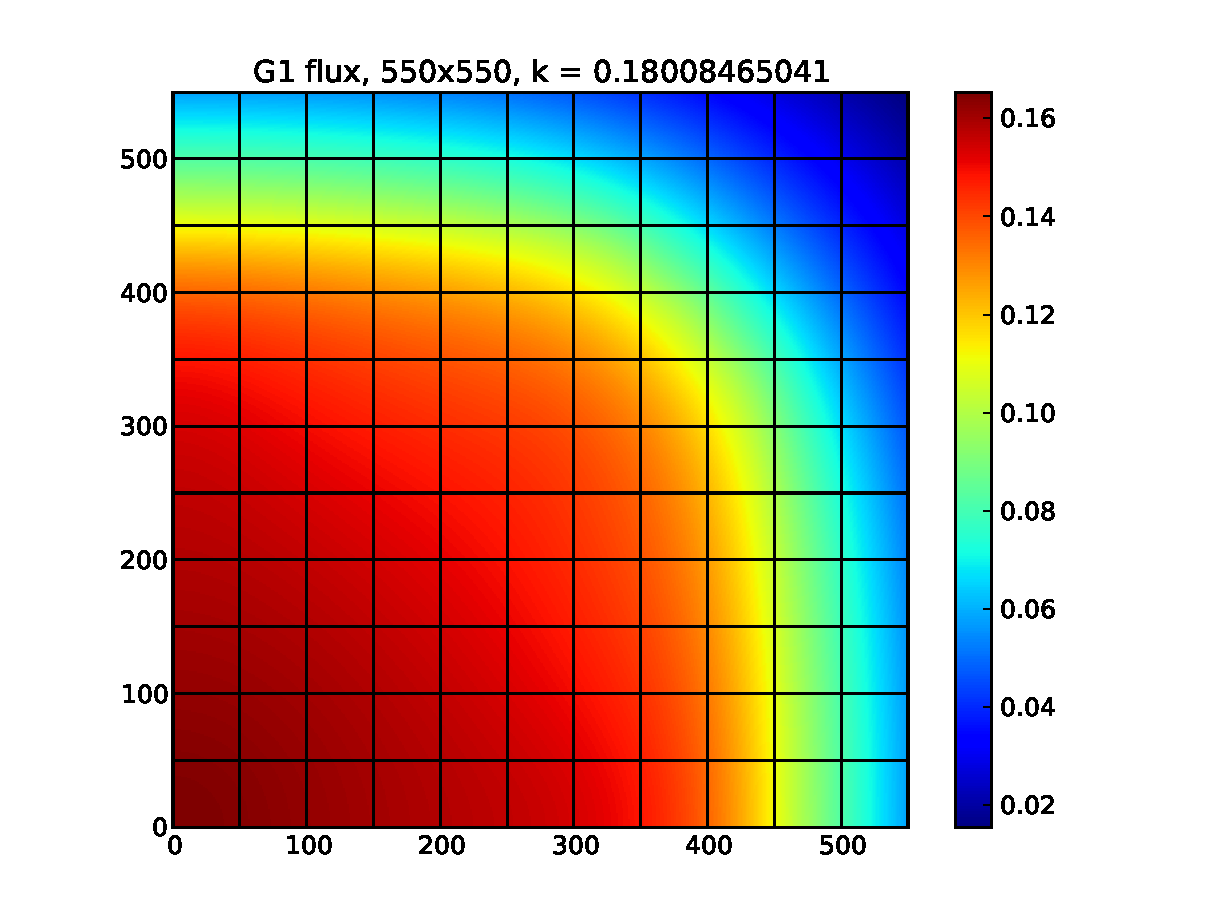
\includegraphics[width=0.45\textwidth]{g1_50_flux} \caption{$N=1$, PLACEHOLDER pdf} \label{kpdf_1}
%\end{figure} \begin{figure}[H] 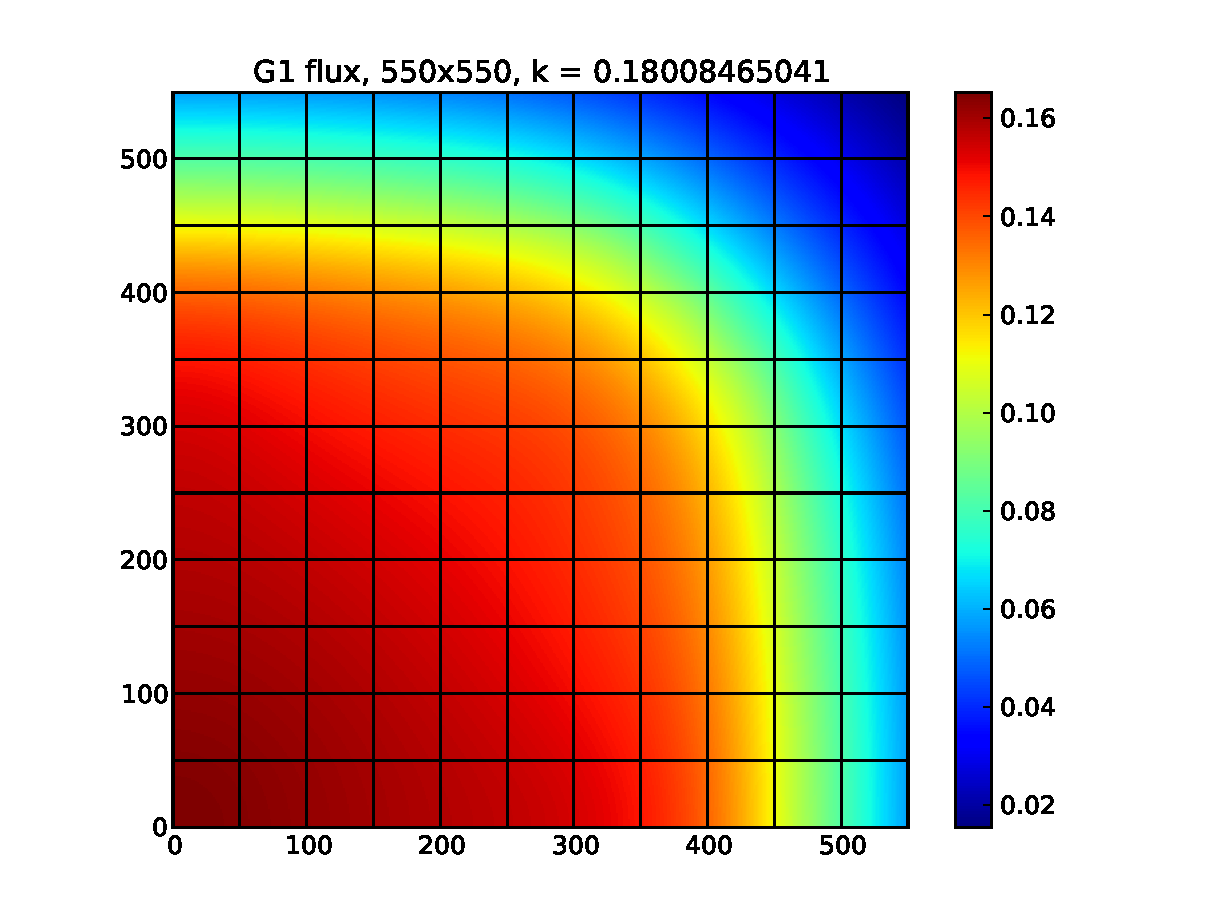
\includegraphics[width=0.45\textwidth]{g1_50_flux} \caption{$N=3$, PLACEHOLDER
%pdf} \label{kpdf_3} \end{figure} \begin{figure}[H] 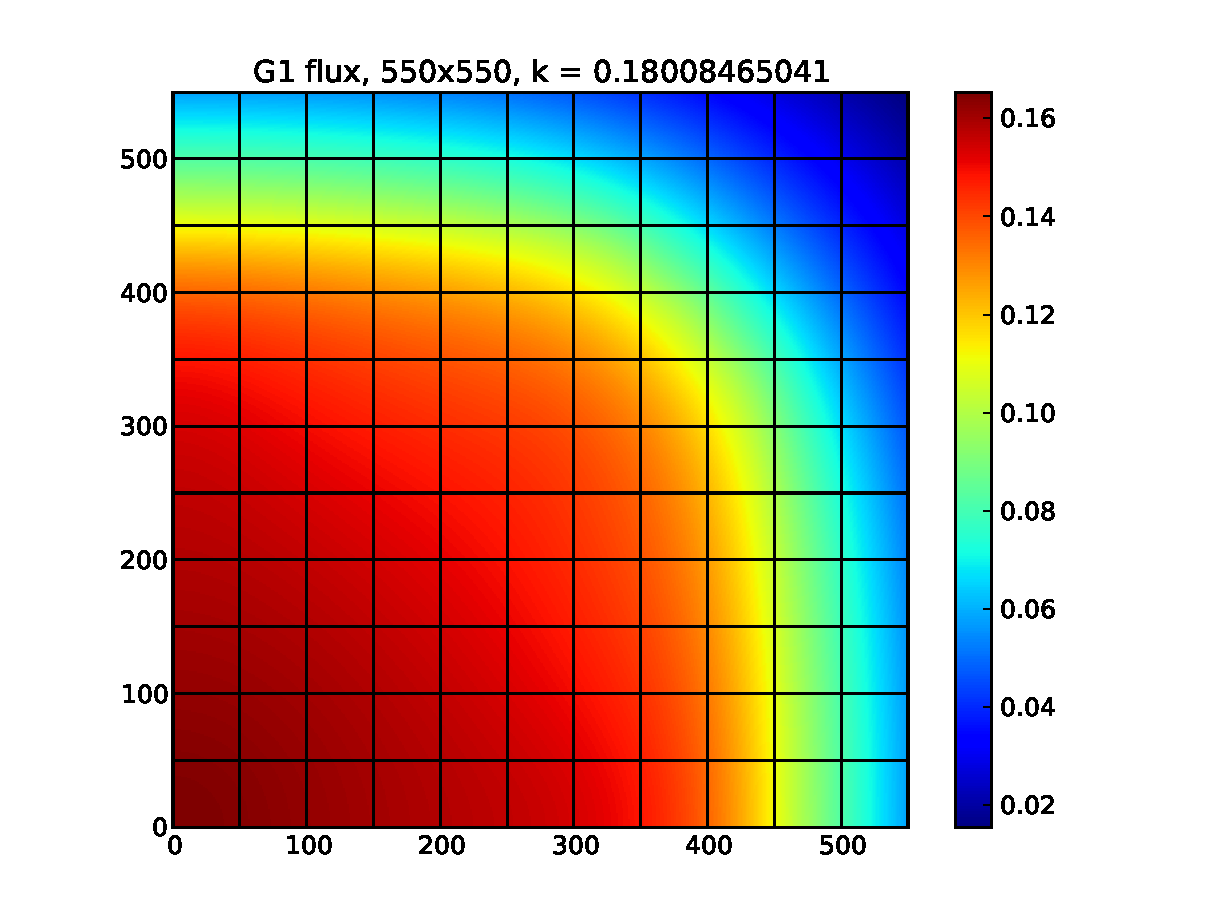
\includegraphics[width=0.45\textwidth]{g1_50_flux}
%\caption{$N=5$, PLACEHOLDER pdf} \label{kpdf_5} \end{figure}
  
  \begin{figure}[htb] 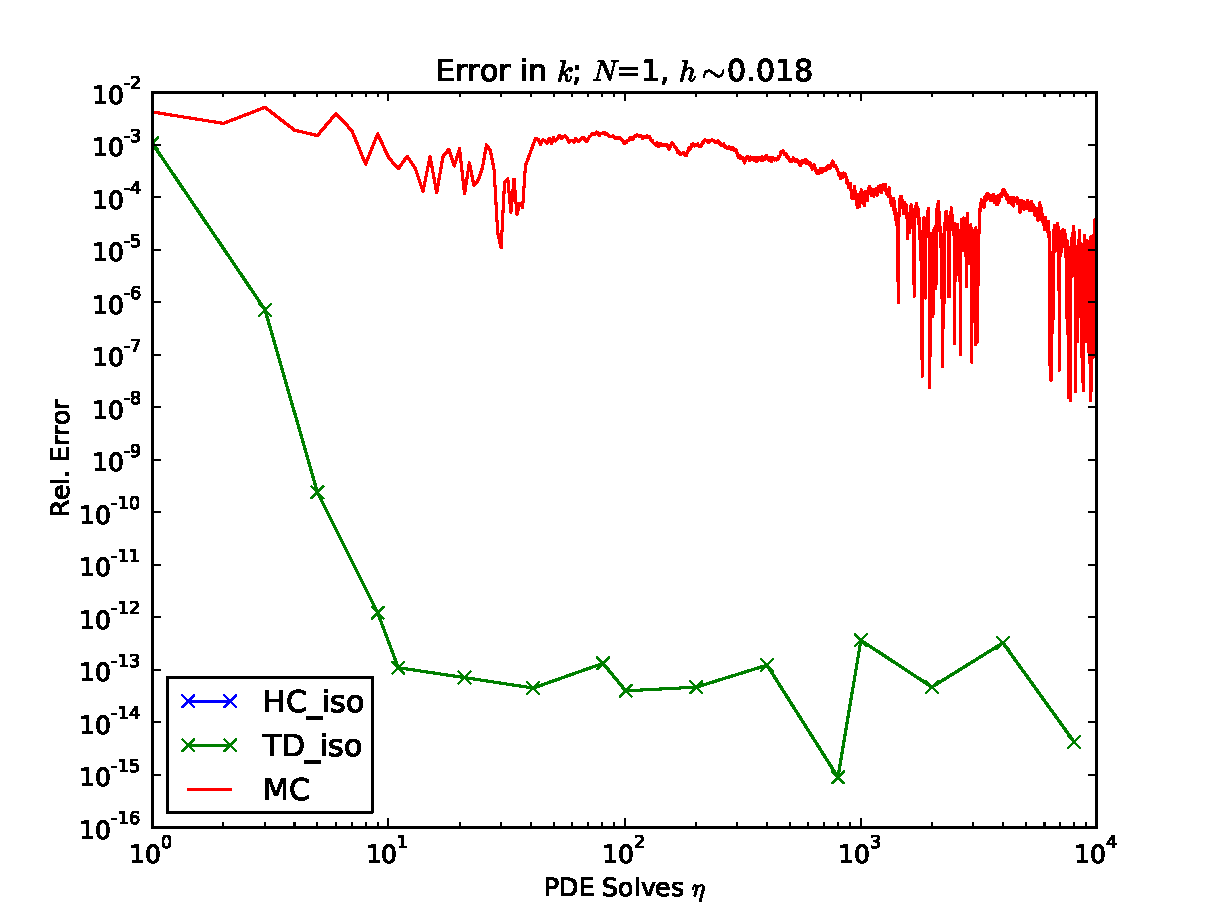
\includegraphics[width=0.45\textwidth]{../graphics/N1_h5_MCHC} \caption{$N=1$, Mean}
    \label{n1mean} \end{figure} \begin{figure}[htb]
    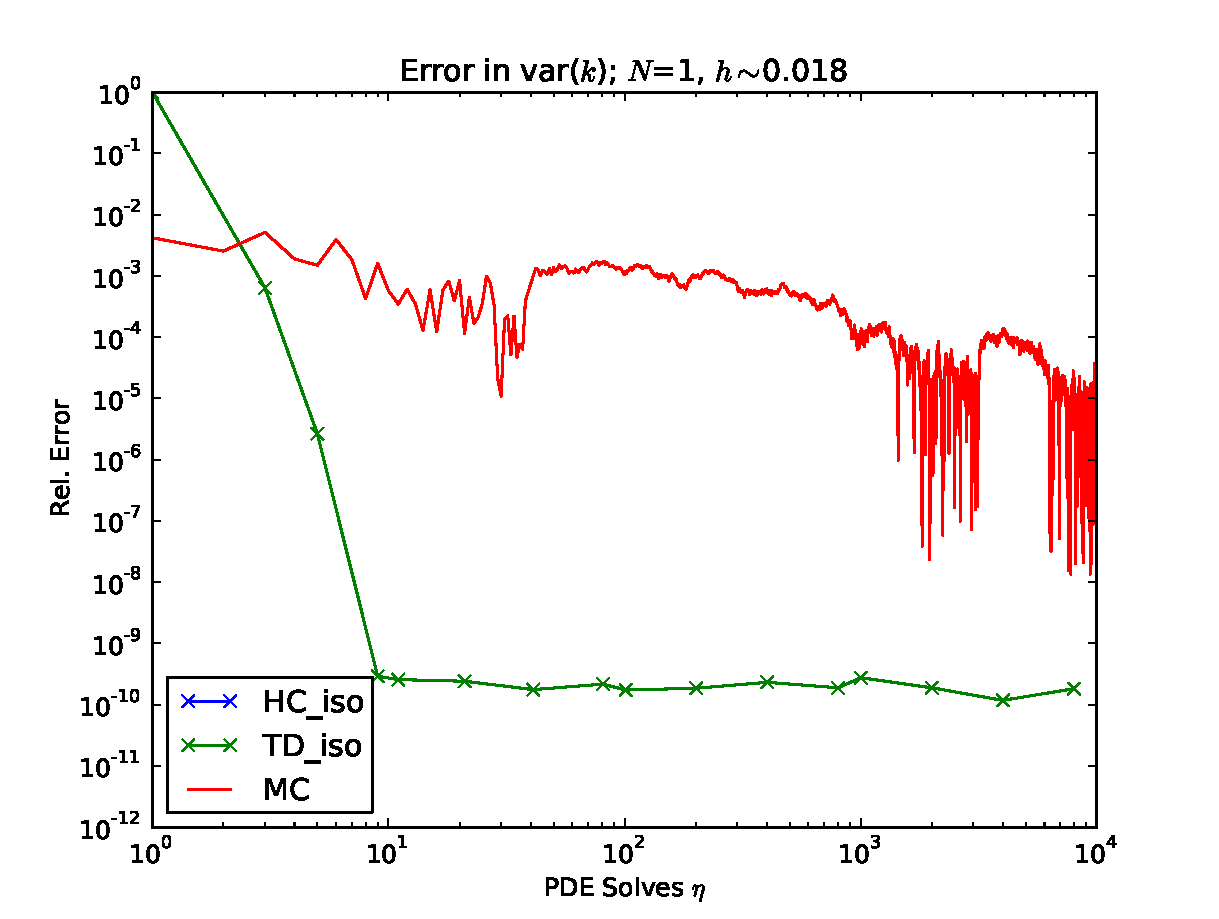
\includegraphics[width=0.45\textwidth]{../graphics/N1_h5_MCHC_2} \caption{$N=1$, Variance} \label{n1var}
  \end{figure}

  \begin{figure}[htb] 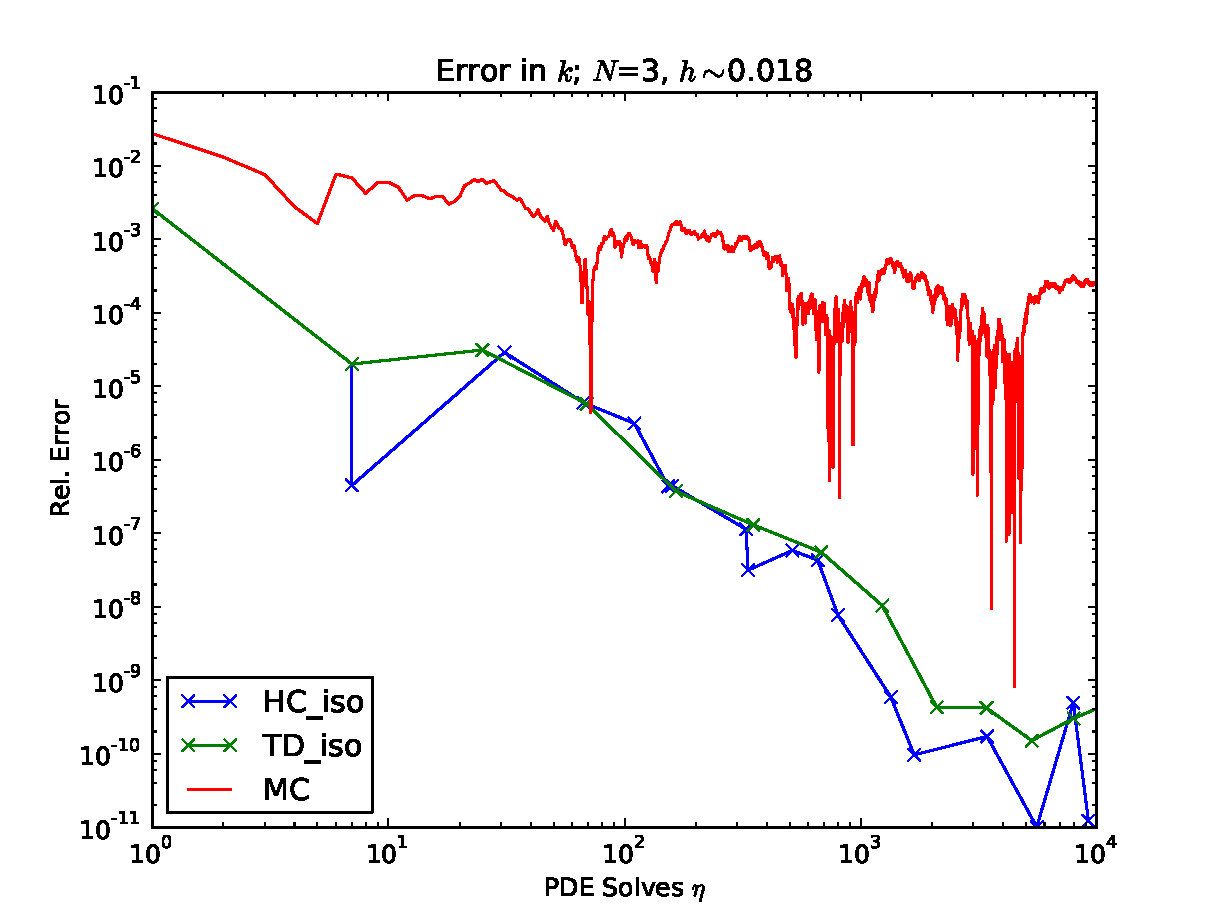
\includegraphics[width=0.45\textwidth]{../graphics/N3_h5_MCHC} \caption{$N=3$, Mean}
    \label{n3mean} \end{figure} \begin{figure}[htb]
    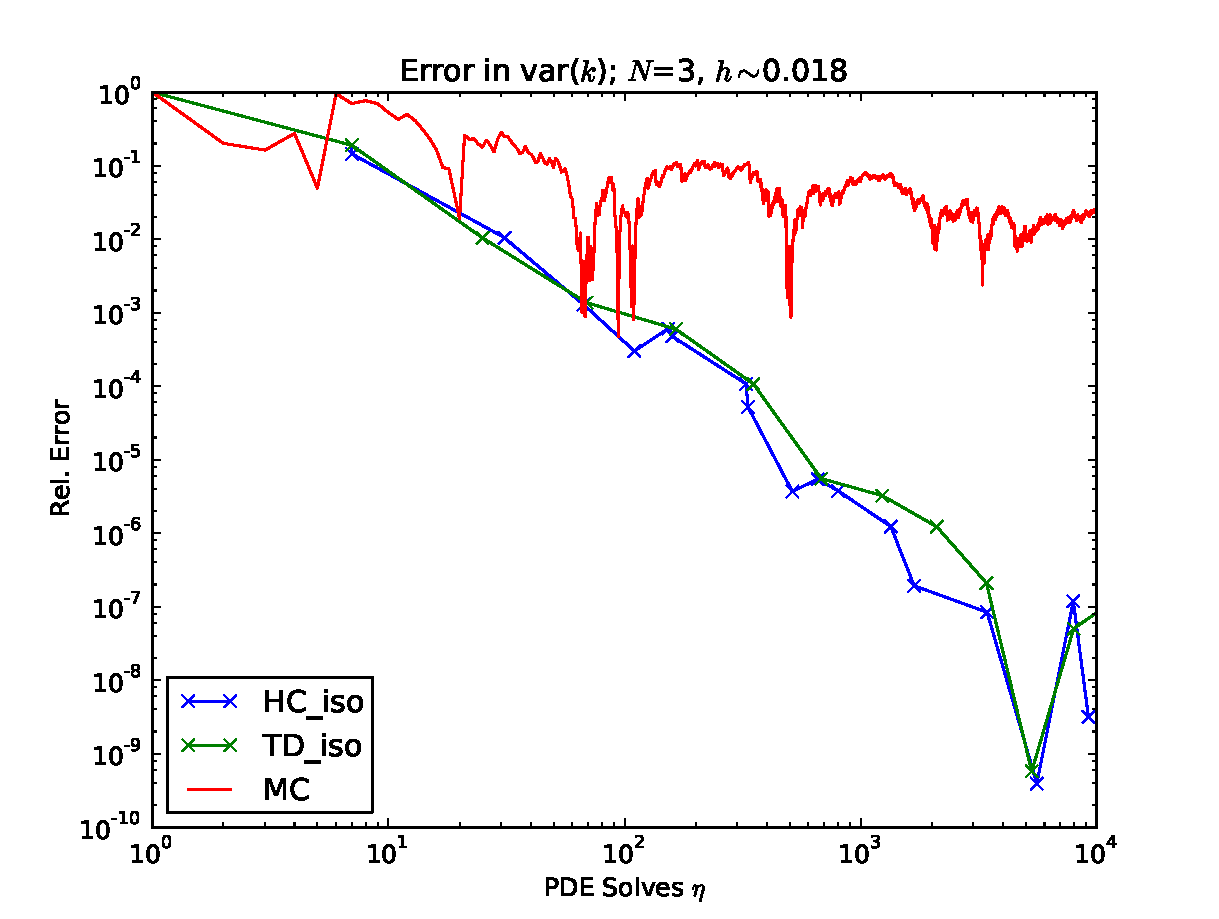
\includegraphics[width=0.45\textwidth]{../graphics/N3_h5_MCHC_2} \caption{$N=3$, Variance} \label{n3var}
  \end{figure}


  \begin{figure}[htb] 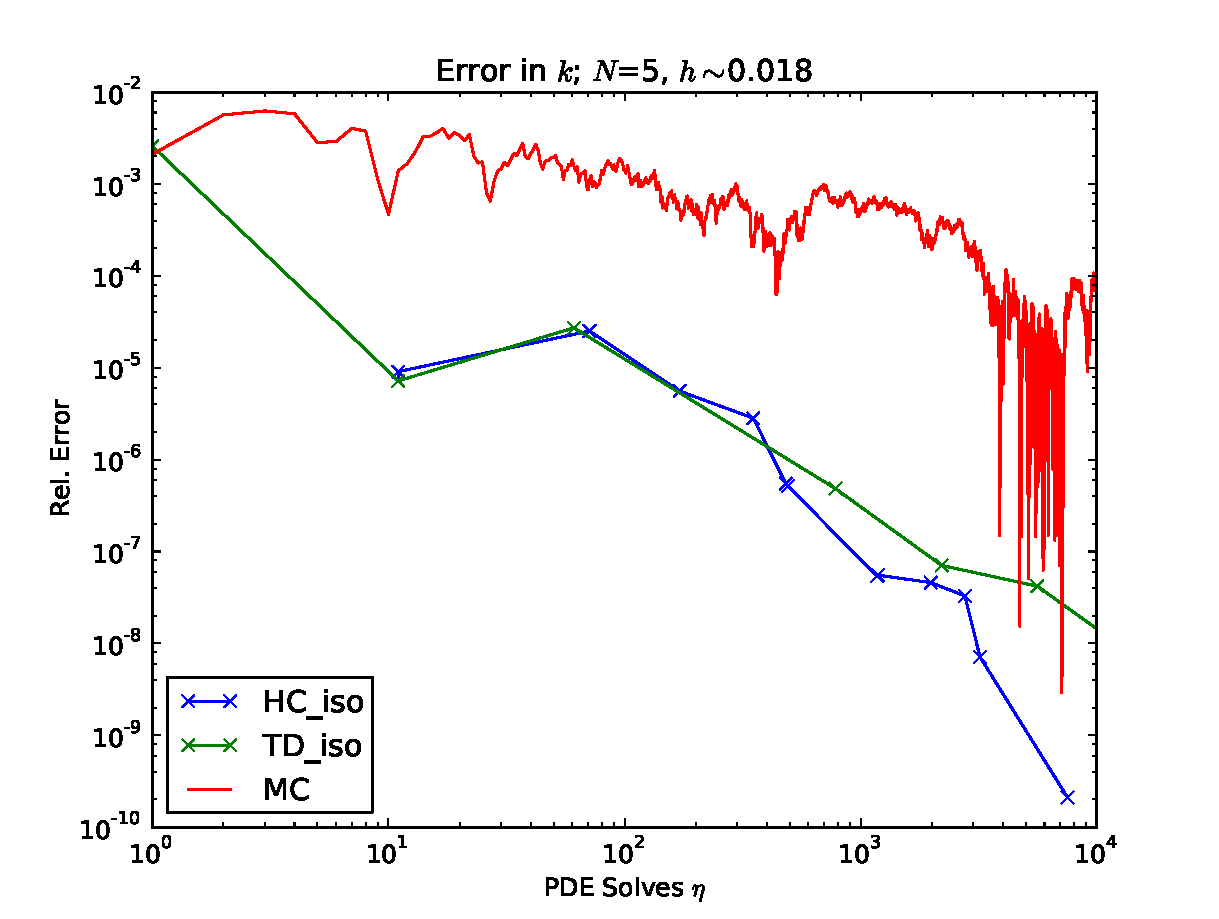
\includegraphics[width=0.45\textwidth]{../graphics/N5_h5_MCHC} \caption{$N=5$, Mean}
    \label{n5mean} \end{figure} \begin{figure}[htb]
    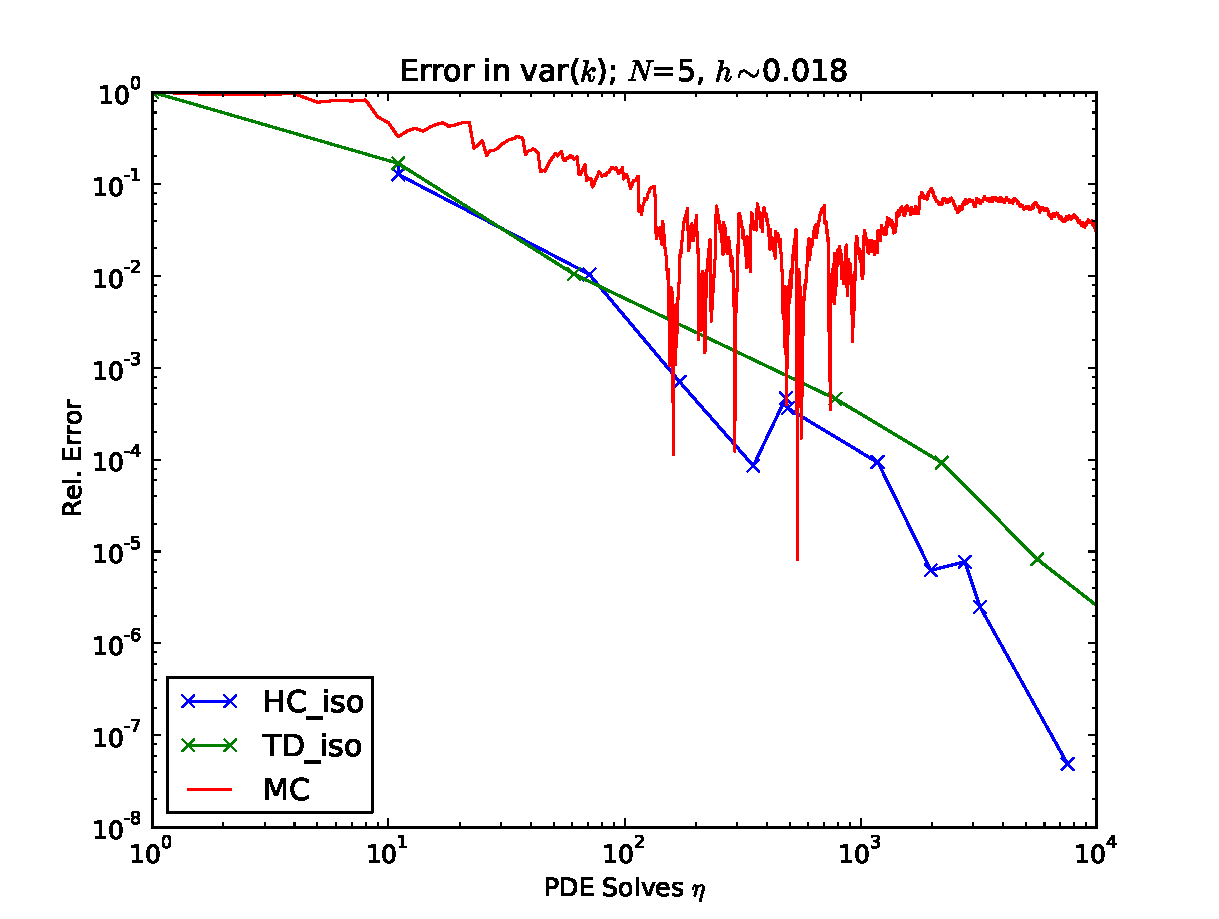
\includegraphics[width=0.45\textwidth]{../graphics/N5_h5_MCHC_2} \caption{$N=5$, Variance} \label{n5var}
  \end{figure}
  
\subsection{Anisotropic Sparse Grid} We present four sets of importance choices and the effect on absolute
error and convergence, along with Monte Carlo and isotropic sparse grids.  Each case is labeled by its
importance weights in order of the input parameters listed in Table \ref{params}, each considering $N=5$
uncertain inputs. The choice of weights is informed by considering the convergence rate varying each
individual parameter alone.  We choose the sample cases $\alpha=(1,1,2,2,4)$ and $\alpha=(1,1,4,4,8)$ to put
increasing weight on the material 1 cross sections and remove weight from the material 5 diffusion
coefficient.  In addition, we intentionally choose a poor weighting scheme with $\alpha=(4,4,2,2,1)$ to show
worst-case effects of including importance weights.  The results are compared in Figs. \ref{aniso1} and
\ref{aniso2} for the mean and variance. 
%\begin{figure}[H] \centering 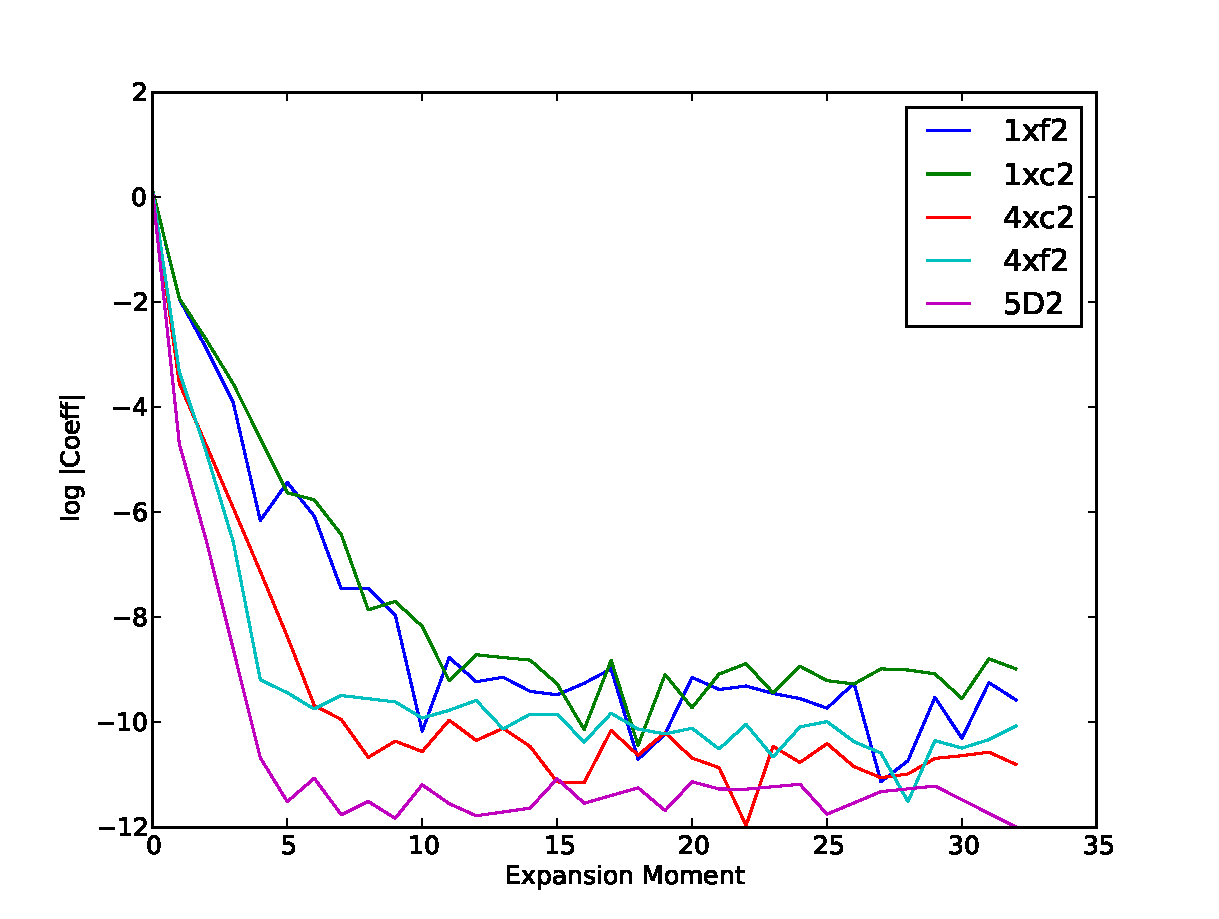
\includegraphics[width=0.45\textwidth]{coefficient_decay2} \caption{Independent
%Stochastic Convergence} \label{indconv} \end{figure}

  \begin{figure}[htb] 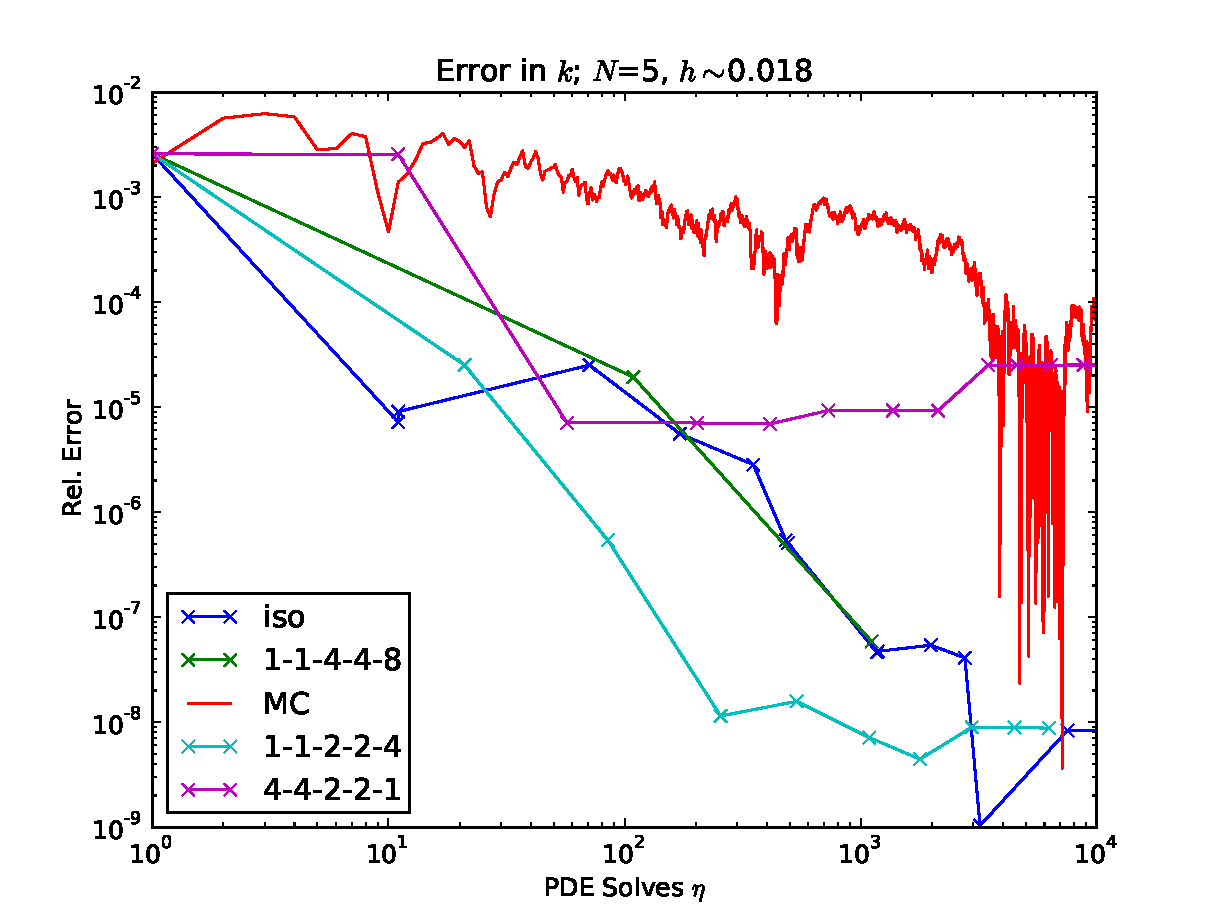
\includegraphics[width=0.45\textwidth]{../graphics/N5_h5_aniso1} \caption{Anisotropic,
    Mean} \label{aniso1} \end{figure} \begin{figure}[htb]
    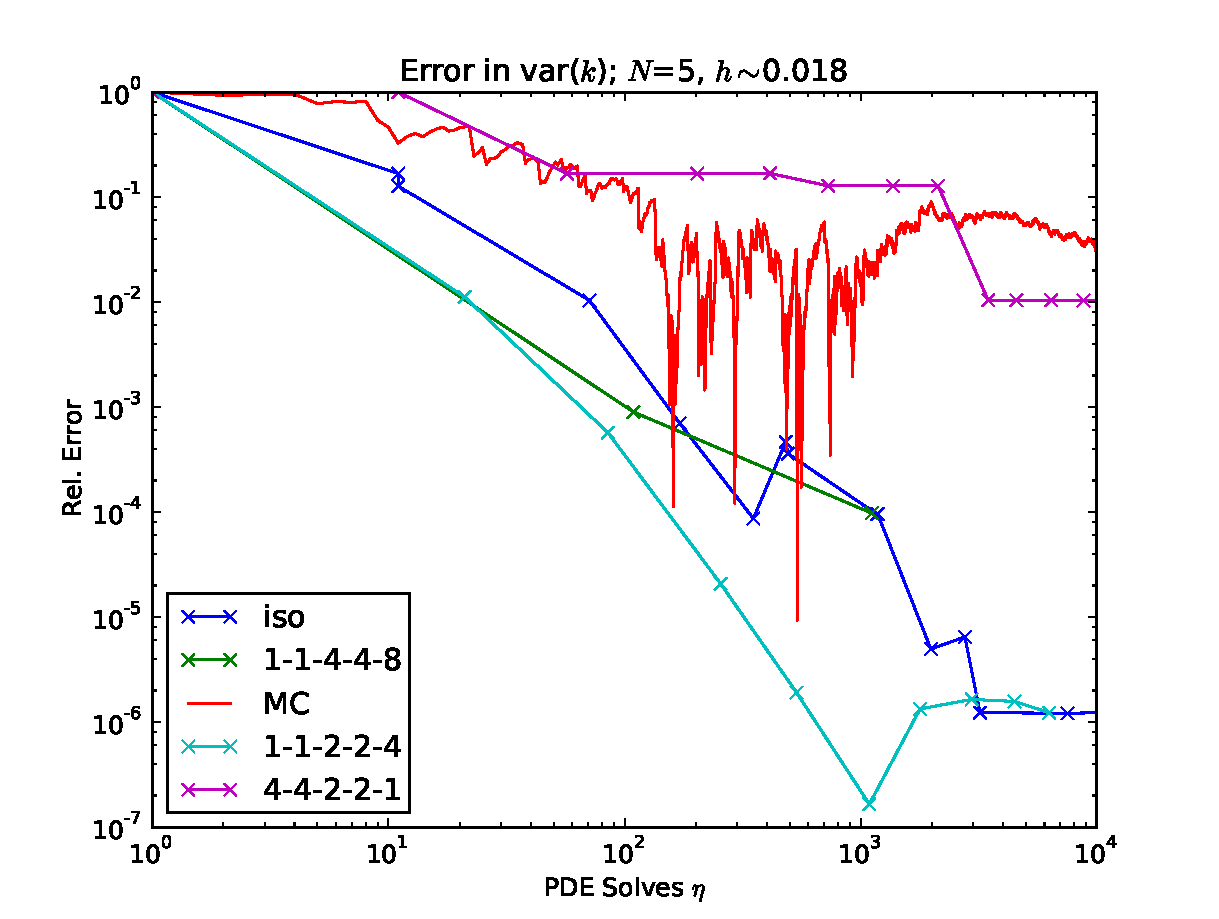
\includegraphics[width=0.45\textwidth]{../graphics/N5_h5_aniso2} \caption{Anisotropic, Variance}
    \label{aniso2} \end{figure}



\section{Discussion} We make a few considerations in analyzing our results.  First, there is a correlation
between the iterative tolerance of the deterministic solver and the maximum convergence of uncertainty
quantification.  If the deterministic space is poorly resolved, it limits the possible convergence in
stochastic space.
%First, there is a noticeable plateau in error convergence in many of the stochastic collocation plots.  This
%seems to be an artifact of the algorithm, which uses an iterative tolerance of $\Delta k <1\times10^{-6}$.
%Because the deterministic solver is only accurate to 6 orders of magnitude, the accuracy of the stochastic
%solver is limited by this value.  We expect reducing the deterministic tolerance to result in further
%possible convergence in stochastic space. 

Additionally, the number of PDE solves for stochastic collocation is determined based on the maximum expansion
level $L$.  For higher $N$, increasing $L$ by only one value increases the number of PDE solves much more than
increasing $L$ by one for small $N$.  As a result, there are few data points to power fit for $N=5$, and the
plateau just mentioned around $\epsilon=10^{-8}$ is more difficult to distinguish from standard convergence.
Resolving the issues leading to the plateau should also resolve this difficulty in fitting points.

We can see the possible benefit and harm of applying importance weighting to an anisotropic grid in Figs.
\ref{aniso1} and \ref{aniso2}.  Any application of anisotropic sparse grids in line with our heuristic
assessment significantly improves the magnitude of error for a given number of PDE solves.  We note, however,
that the convergence of $\alpha=(1,1,2,2,4)$ is better than the more extreme $\alpha=(1,1,4,4,8)$.  This
suggests that with $\alpha=(1,1,2,2,4)$ we have achieved an optimum efficiency that isn't improved with
further anisotropy.  However, the anisotropy intentionally chosen poorly, $\alpha=(4,4,2,2,1)$, shows much
worse convergence than the isotropic case, and for the variance is on par with Monte Carlo.  Given these
limitations, it is clear that for the uncertain spaces presented, stochastic collocation shows much better
convergence and magnitude of error for the same cost when compared with Monte Carlo. 

%\section{Ongoing Work} The work presented here considers a maximum number of uncertain variables $N=5$.
%While demonstrative of expected savings for larger input spaces, showing the convergence rates of isotropic
%and anisotropic sparse grids for large $N$ is desirable.  We expect to see diminishing returns in using
%stochastic collocation as the input space grows in dimensionality.\\
%
%One effective method for very large numbers of uncertain inputs is HDMR, which uses sets of low-order
%stochastic interactions between a few variables at a time to approximate the full stochastic problem.  In the
%event the number of uncertain parameters becomes very large, HDMR could prove less costly than stochastic
%collocation for many problems. \\
%
%Lastly, our work so far has been demonstrated exclusively with uniformly-distributed random variables as
%input parameters.  To more accurately approximate the shape of an arbitrary probability distribution, we
%intend to implement Beta-distributed random variables using Jacobi quadrature, with two shaping parameters
%$\alpha,\beta$.  The Beta distribution is also distributed finitely between two points, but $\alpha,\beta$
%can be adjusted to accommodate a wide range of uncertain distributions including uniform and truncated
%Gaussian normal distributions.  While Beta distributions cannot exactly replicate all other distributions, we
%expect it can replicate them without introducing a greater error than introduced by the Monte Carlo and
%stochastic collocation methods presented.

%\newpage
\bibliography{../bibliography/uq}{} \bibliographystyle{plain} \end{document}
